\section{System Overview}
\subsection{Definitions}

\begin{description}
    \item[Processor]
    \hfill\\
    The processor implementation on the FPGA.
    \item[Board]
    \hfill\\
    The printed circuit board (PCB).
    \item[Computer]
    \hfill\\
    The board with soldered components.
    \item[System]
    \hfill\\
    The computer with peripherals, power supply, etc.
\end{description}



\begin{figure}[h]
    \centering
    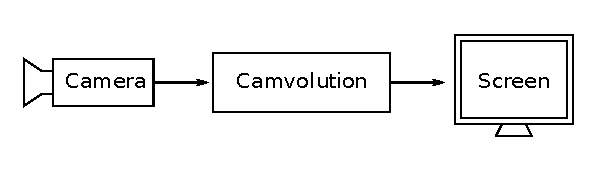
\includegraphics{img/SystemOverview.pdf}
    \caption{System Overview}
    \label{fig:SystemOverview}
\end{figure}

As stated in the introduction, we want our system to perform convolution on a live video stream.
This is visualized in Figure \ref{fig:SystemOverview}.
The video stream flows into our system from an external source, preferably a camera as depicted in the figure.
Then our system performs the convolution and passes the image on to an external display, in this case a screen.
As stated in the requirements, the system should handle streaming video from a camera, perform convolution and be able to provide the result as an output stream.

\subsection{Implementation}
The convolution is to be done on the FPGA using a custom processor implementation described in Section \ref{sec:processor}.
First of all, this satisfies non-functional requirement NFR1.
Secondly, this allows us to do hardware accelerated convolution, which will hopefully make it possible to achieve the speeds we have in mind.
Thirdly, this demonstrates how an FPGA can be used as reconfigurable hardware to accelerate application specific tasks.

This configuration of the FPGA is going to be done by the MCU, which will fetch the configuration from an SD card so that the configuration can be easily exchanged for a different one to harvest the advantages of reconfigurable hardware.

In addition to configuring the FPGA, the MCU should also handle the input stream arriving from a camera or another external video source.
As convolution is done on the FPGA, the MCU should forward the video stream to the FPGA and possibly perform some preprocessing should the video format from the camera be unsuitable for our core on the FPGA.
This may include indexing the colours or reducing the colour depth to a different colour representation as described in Section \ref{sec:DigitalVideo} which may be necessary to speed up the processing and reduce throughput.

Connected to the FPGA is also some extra memory as the internal memory on the FPGA is limited in size.
This memory in supposed to work as a buffer to make the system more tolerable to variable data bit rates and to allow the output to read old data while waiting for the processed input to arrive.

As HDMI output is not available on the MCU and the bus between the MCU and FPGA is already assumed to be a bottleneck, the HDMI output is placed on the FPGA.
The final data flow through the system can be seen in Figure \ref{fig:SystemArchitecture}.

Figure \ref{fig:SystemArchitecture} displays the overall data flow between the components in the system.
Notice that most of the data flows from the left to the right. Video arrives through the camera and flows through the system all the way to the HDMI output, FPGA configurations flow from the SD card through the MCU to the FPGA on configuration.

\begin{figure}
    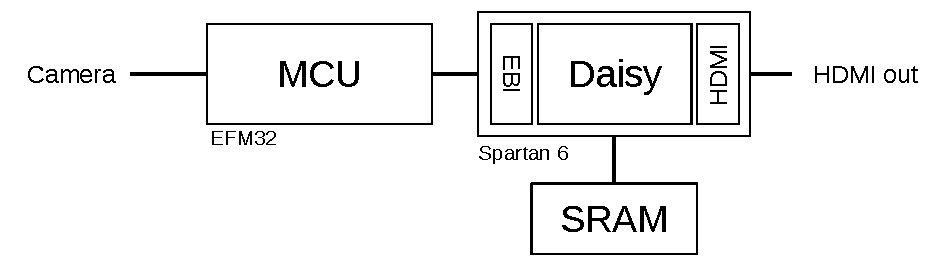
\includegraphics{img/SystemArchitecture}
    \caption{Video Data Flow}
    \label{fig:SystemArchitecture}
\end{figure}

\subsection{Backup Solutions} \label{subsec:RiskAssessment}
During the project, a risk assessment was done to find and reduce the risk of failure.
This lead to some backup solutions being implemented in the design.

One such solution was to exaggerate the number of address lines from the MCU to the FPGA to support addressing the memory connected to the FPGA directly (through the FPGA).
This will be useful should the communication directly from the MCU to the processor prove hard to establish.
This is a critical point because the data needs to cross clock domains correctly.

One of the measures taken was to add an extra HDMI port connected to the FPGA in case we failed to transfer video from the MCU to the FPGA or the throughput proved to be insufficient.
This allows us to connect the camera directly to the FPGA and circumvent both the MCU and the bus between the MCU and FPGA, as shown in Figure \ref{fig:SystemArchitectureAlternative}
In addition, a connector for a Raspberry Pi camera (FPC) exists for connecting a camera to the FPGA.

Should all camera input strategies fail, video or images can be loaded from the SD card or generated by the MCU.

Also shown in Figure \ref{fig:SystemArchitectureAlternative} is an extra SRAM chip.
The extra chip doubles the available throughput between the memory and the FPGA and reduces the chance of conflicts between the processor and the HDMI controller which will access the memory at the same time. Using double buffering, we can ensure they never access the same memory at the same time.

Header pins for VGA output was also added to the FPGA in case we ended up being unable to output HDMI correctly.

\begin{figure}
    \centering
    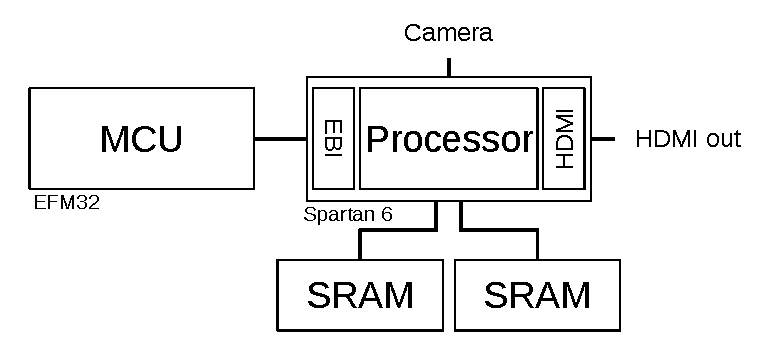
\includegraphics{img/SystemArchitectureAlternative.pdf}
    \caption{Alternative System Architecture}
    \label{fig:SystemArchitectureAlternative}
\end{figure}
